
\documentclass[notheorems,serif]{beamer}

%选用主题
%\usetheme{Rochester}
%\usetheme{default}
%\usetheme{AnnArbor}
%\usetheme{Antibes}
%\usetheme{Bergen}
%\usetheme{Berkeley}
%\usetheme{Berlin}
%\usetheme{Boadilla}
%\usetheme{CambridgeUS}
%\usetheme{Copenhagen}
%\usetheme{Darmstadt}
%\usetheme{Dresden}
%\usetheme{Frankfurt}
%\usetheme{Goettingen}%
%\usetheme{Hannover}
%\usetheme{Ilmenau}
%\usetheme{JuanLesPins}
%\usetheme{Luebeck}
\usetheme{Madrid}
%\usetheme{Malmoe}
%\usetheme{Marburg}
%\usetheme{Montpellier}
%\usetheme{PaloAlto}
%\usetheme{Pittsburgh}
%\usetheme{Rochester}
%\usetheme{Singapore}
%\usetheme{Szeged}
%\usetheme{Warsaw}

% As well as themes, the Beamer class has a number of color themes
% for any slide theme. Uncomment each of these in turn to see how it
% changes the colors of your current slide theme.

%\usecolortheme{albatross}
%\usecolortheme{beaver}
%\usecolortheme{beetle}
%\usecolortheme{crane}
%\usecolortheme{dolphin}
%\usecolortheme{dove}
%\usecolortheme{fly}
%\usecolortheme{lily}
%\usecolortheme{orchid}
%\usecolortheme{rose}
%\usecolortheme{seagull}
%\usecolortheme{seahorse}
%\usecolortheme{whale}
%\usecolortheme{wolverine}

%设置被cover的内容不显示
%\setbeamercovered{transparent}

\useinnertheme{rounded}
\usecolortheme{default}

%调用包
\usepackage[no-math, cm-default]{fontspec}
\usepackage{xltxtra}
\usepackage{xunicode}   
\usepackage{xcolor}
\usepackage{amsmath,amssymb}
\usepackage{xeCJK}
\usepackage{multimedia}
\usepackage{listings}
\usepackage{subfigure}
\usepackage{todonotes}
\presetkeys{todonotes}{inline}{} 
\usepackage{multicol}
\usepackage{changes}




%将系统字体名映射为逻辑字体名称,主要是为了维护的方便  
\newcommand\fnhei{Adobe 黑体 Std}  
\newcommand\fnsong{Adobe 宋体 Std}  
\newcommand\fnkai{Adobe 楷体 Std}  
\newcommand\fnmono{DejaVu Sans Mono}  
\newcommand\fnroman{Times New Roman}  

\renewcommand{\normalsize}{\wuhao}

%%设置常用中文字号,方便调用  
\newcommand{\erhao}{\fontsize{22pt}{\baselineskip}\selectfont}  
\newcommand{\xiaoerhao}{\fontsize{18pt}{\baselineskip}\selectfont}  
\newcommand{\sanhao}{\fontsize{16pt}{\baselineskip}\selectfont}  
\newcommand{\xiaosanhao}{\fontsize{15pt}{\baselineskip}\selectfont}  
\newcommand{\sihao}{\fontsize{14pt}{\baselineskip}\selectfont}  
\newcommand{\xiaosihao}{\fontsize{12pt}{\baselineskip}\selectfont}  
\newcommand{\wuhao}{\fontsize{10.5pt}{\baselineskip}\selectfont}  
\newcommand{\xiaowuhao}{\fontsize{9pt}{\baselineskip}\selectfont}  
\newcommand{\liuhao}{\fontsize{7.5pt}{\baselineskip}\selectfont}  

%\setmainfont{\fnroman}
\setmainfont{\fnkai}
\setCJKmainfont[BoldFont=\fnhei]{\fnkai}  
\setCJKsansfont[BoldFont=\fnhei]{\fnkai}  
\setCJKmonofont{\fnkai}  

%楷体  
%\newfontinstance\KAI{\fnkai}  
%\newcommand{\kai}[1]{{\KAI#1}}  
%黑体  
%\newfontinstance\HEI{\fnhei}  
%\newcommand{\hei}[1]{{\HEI#1}}  
%英文  
%\newfontinstance\ENF{\fnroman}  
%\newcommand{\en}[1]{\,{\ENF#1}\,}

%楷体  
\newfontfamily\KAI {\fnkai}  
\newcommand{\kai}[1]{{\KAI#1}}  
%黑体  
\newfontfamily\HEI{\fnhei}  
\newcommand{\hei}[1]{{\HEI#1}}  
%英文  
\newfontfamily\ENF{\fnroman}  
\newcommand{\en}[1]{\,{\ENF#1}\,}


%连字符
\defaultfontfeatures{Mapping=tex-text}

%中文断行
\XeTeXlinebreaklocale "zh"
\XeTeXlinebreakskip = 0pt plus 1pt minus 0.1pt


%%%% 定理类环境的定义 %%%%
\newtheorem{example}{\hei{例子}} 
\newtheorem{problem}{\hei{问题}}           
\newtheorem{algorithm}{\hei{算法}}
\newtheorem{theorem}{\hei{定理}}
\newtheorem{definition}{\hei{定义}}
\newtheorem{axiom}{\hei{公理}}
\newtheorem{property}{\hei{性质}}
\newtheorem{proposition}{\hei{命题}}
\newtheorem{lemma}{\hei{引理}}
\newtheorem{corollary}{\hei{推论}}
\newtheorem{remark}{\hei{注解}}
\newtheorem{condition}{\hei{条件}}
\newtheorem{conclusion}{\hei{结论}}
\newtheorem{assumption}{\hei{假设}}

%重定义一些环境的名字
\renewcommand{\proofname}{\hei{证明}}
\renewcommand\tablename{\hei{表}}
%---SCRIPT-----------------------------------------------------------------------------------------
\newcommand{\cA}{\mathcal{A}}
\newcommand{\cB}{\mathcal{B}}
\newcommand{\cC}{\mathcal{C}}
\newcommand{\cD}{\mathcal{D}}
\newcommand{\cE}{\mathcal{E}}
\newcommand{\ce}{\mathcal{e}}
\newcommand{\cF}{\mathcal{F}}
\newcommand{\cG}{\mathcal{G}}
\newcommand{\cg}{\mathcal{g}}
\newcommand{\cH}{\mathcal{H}}
\newcommand{\cI}{\mathcal{I}}
\newcommand{\cJ}{\mathcal{J}}
\newcommand{\cK}{\mathcal{K}}
\newcommand{\cL}{\mathcal{L}}
\newcommand{\cM}{\mathcal{M}}
\newcommand{\cN}{\mathcal{N}}
\newcommand{\cO}{\mathcal{O}}
\newcommand{\cP}{\mathcal{P}}
\newcommand{\cQ}{\mathcal{Q}}
\newcommand{\cR}{\mathcal{R}}
\newcommand{\cS}{\mathcal{S}}
\newcommand{\cT}{\mathcal{T}}
\newcommand{\cU}{\mathcal{U}}
\newcommand{\cV}{\mathcal{V}}
\newcommand{\cW}{\mathcal{W}}
\newcommand{\cX}{\mathcal{X}}
\newcommand{\cY}{\mathcal{Y}}
\newcommand{\cZ}{\mathcal{Z}}
\newcommand{\cz}{\mathcal{z}}
%---BLACKBOARD-------------------------------------------------------------------------------------
\newcommand{\mA}{\mathbb A}
\newcommand{\mB}{\mathbb B}
\newcommand{\mC}{\mathbb C}
\newcommand{\mD}{\mathbb D}
\newcommand{\mE}{\mathbb E}
\newcommand{\mF}{\mathbb F}
\newcommand{\mG}{\mathbb G}
\newcommand{\mg}{\mathbb g}
\newcommand{\mH}{\mathbb H}
\newcommand{\mI}{\mathbb I}
\newcommand{\mJ}{\mathbb J}
\newcommand{\mK}{\mathbb K}
\newcommand{\mL}{\mathbb L}
\newcommand{\mM}{\mathbb M}
\newcommand{\mN}{\mathbb N}
\newcommand{\mO}{\mathbb O}
\newcommand{\mP}{\mathbb P}
\newcommand{\mQ}{\mathbb Q}
\newcommand{\mR}{\mathbb R}
\newcommand{\mS}{\mathbb S}
\newcommand{\mT}{\mathbb T}
\newcommand{\mU}{\mathbb U}
\newcommand{\mV}{\mathbb V}
\newcommand{\mW}{\mathbb W}
\newcommand{\mX}{\mathbb X}
\newcommand{\mY}{\mathbb Y}
\newcommand{\mZ}{\mathbb Z}
\newcommand{\mz}{\mathbb z}

\newcommand{\bV}{\mathbf{V}}
\newcommand{\bz}{\mathbf{z}}
\newcommand{\bT}{\mathbf{T}}
\newcommand{\bx}{\mathbf{x}}
\newcommand{\be}{\mathbf{e}}
\newcommand{\bff}{\mathbf{f}}
\newcommand{\bg}{\mathbf{g}}
\newcommand{\bn}{\mathbf{n}}
\newcommand{\bt}{\mathbf{t}}
\newcommand{\bd}{\mathbf{d}}
\newcommand{\bzero}{\mathbf{0}}
\newcommand{\bka}{\mathbf{\kappa}}

\newcommand{\rd}{\mathrm{d}}
%---SHORTCUTS--------------------------------------------------------------------------------------
\newcommand\xor{\mathbin{\char`\^}}
\DeclareMathOperator{\res}{Res}
\DeclareMathOperator{\sgn}{sgn}
\DeclareMathOperator{\supp}{supp}
\DeclareMathOperator{\as}{as}
\newcommand{\slant}[1]{\slshape #1\normalfont}
\newcommand{\dd}[2]{\frac{d#1}{d#2}} 
\newcommand{\ddx}{\frac{d}{dx}}
\newcommand{\ddt}{\frac{d}{dt}}
\newcommand{\dds}{\frac{d}{ds}}
\newcommand{\pd}[1]{\ds\frac{\partial}{\partial #1 }}
\newcommand{\pdd}[2]{\ds\frac{\partial #1}{\partial #2 }}
\newcommand{\mdd}[3]{\ds\frac{\partial^{#3} #1}{\partial #2^{#3} }}
\newcommand{\x}{\ _\Box}
\newcommand{\ds}{\displaystyle}
\newcommand{\bs}{\backslash}
\newcommand{\Bold}{\noindent \bfseries}
\newcommand{\Norm}{\normalfont}
\newcommand{\exl}[1]{\textcolor{NavyBlue}{\Bold Exercise #1 \Norm}}
\newcommand{\ex}{\textcolor{NavyBlue}{\Bold Problem: \Norm}}
\newcommand{\sol}{\textcolor{Mulberry}{\Bold Solution: \Norm}}
\newcommand{\pf}{\textcolor{Mulberry}{\Bold Proof: \Norm}}
\newcommand{\Title}[1]{\LARGE\Bold \textcolor{Sepia}{#1}\Norm\normalsize \vspace{10pt} \newline}
\newcommand{\prop}{\Bold \textcolor{YellowOrange}{ Proposition:} \Norm}
\newcommand{\propl}[1]{\Bold \textcolor{YellowOrange}{ Proposition #1:} \Norm}
\newcommand{\rk}{\Bold \textcolor{YellowOrange}{ Remark:} \Norm}
\newcommand{\rmk}[1]{\Bold\textcolor{YellowOrange}{#1} \Norm}
\newcommand{\thm}[1]{\Bold \textcolor{YellowOrange}{ Theorem #1} \Norm}
\newcommand{\ind}{\indent\indent}
\newcommand{\br}{\vspace{10pt} \newline}

\newcommand{\red}{\color{red}}
\newcommand{\blue}{\color{blue}}


\begin{document}
\title[数值线性代数]{{\small\leftline{数值线性代数———}~~~~~~~~~~~~~~~~~~~~~~~~~~~~~~~~~~~~~~~~~~~~~~
~~~~~~~~~~~} \\
矩阵计算
}




\author[]{~~潘建瑜~~}

\institute[湘潭大学数学系]

\date[\today]

%\pgfdeclareimage[height=1cm]{institution-logo}{figures/xtu.pdf}

%\logo{\pgfuseimage{institution-logo}}


\frame[plain]{\titlepage}


\AtBeginSection[]{

  \frame<beamer>{ 

    \frametitle{线性方程组的迭代解法}   

    \tableofcontents[currentsection] 

  }
}

\begin{frame}
\large 方法综述
\normalsize
\begin{itemize}
   \item {\color{blue}直接法}\quad PLU分解, LDLT分解, Cholesky分解法
   
   \item {\color{blue}迭代法}
   
         
         
         -Krylov子空间迭代法: CG, MIRES, GMRES, BiCGStab等
   
   \item {\color{blue}快速算法}

         -基于快速变换,如FFT, DCT, DST等

         -代数多重网格法(Algebraic multigrid)

         -快速多极子算法(Fast multipole)

\end{itemize}
有些方法可能只是对某类方程有效,如快速算法.在实际应用中,这些方法可以结合使用,如混合(hybrid)算法,预处理算法(preconditioning)等
\end{frame}



\begin{frame}
\centerline{本讲主要介绍定常迭代算法}
\qquad 

\qquad 

\qquad 

\qquad 

\qquad 

\qquad 


更多迭代方法可参见{\color{blue}Templates for the Solution of Linear Systems:Building Blocks for Iterative Methods,}SLAM,1994
\end{frame}

\newpage
\section{离散Poisson方程}

\begin{frame}
在本讲中,我们以一个典型的线性方程组为例,逐个介绍各种迭代方法,并比较它们之间的性能.这个方程组就是二维Poisson方程经过五点差分离散后得到的线性方程组.
\end{frame}

\begin{frame}\frametitle{一维Poisson方程}
考虑如下带Dirichlet边界条件的一维Poisson方程

\begin{align}
\begin{cases}
	\frac{\mathrm{d^2} u(x)}{\mathrm{d}x^2} =f(x),0<x<1,\\
	u(0)=a,u(1) = b\\
\end{cases}
\tag{6.1}
\end{align}

其中$f(x)$是给定的函数,$u(x)$是需要计算的未知函数.
\end{frame} 

\begin{frame}\frametitle{一维Poisson方程}
{\color{blue}\Large 差分离散}

\quad

\normalsize
取步长$h=\frac{1}{n+1}$,为节点$x_i=ih,i=0,1,2,...,n+1$我们采用中心差分离散,可得$(i=1,2,...,n)$
$$
-\left.\frac{d^{2} u(x)}{d x^{2}}\right|_{x_{i}}=\frac{2 u\left(x_{i}\right)-u\left(x_{i-1}\right)-u\left(x_{i+1}\right)}{h^{2}}+O\left(h^{2} \cdot\left\|\frac{d^{4} u}{d x^{4}}\right\|_{\infty}\right)
$$
将其代入(6.1),舍去高阶项后可得Poisson方程在$x_i$点的近似离散方程
$$\boxed{-u_{i-1}+2u_i-u_{i+1}=h^2f_i,}$$
\end{frame}

\begin{frame}\frametitle{一维Poisson方程}
其中$f_i=f(x_i),u_i$为$u(x_i)$的近似.

令$i= 1,2,...,n,$则可0得$n$个线性方程,写成矩阵形式
\begin{align}
{T_nu=f,}
\tag{6.2}
\end{align}
其中
\begin{equation}
T_{n}=\left[\begin{array}{cccc}{2} & {-1} & {} & {} \\ {-1} & {\ddots} & {\ddots} & {} \\ {} & {\ddots} & {\ddots} & {-1} \\ {} & {} & {-1} & {2}\end{array}\right], u=\left[\begin{array}{c}{u_{1}} \\ {u_{2}} \\ {\vdots} \\ {u_{n-1}} \\ {u_{n}}\end{array}\right], f=\left[\begin{array}{c}{f_{1}+u_{0}} \\ {f_{2}} \\ {\vdots} \\ {f_{n-1}} \\ {f_{n}+u_{n+1}}\end{array}\right]
\tag{6.3}
\end{equation}
\end{frame}

\begin{frame}\frametitle{一维Poisson方程}
{\color{blue}\Large 系数矩阵$T_n$的性质}

\quad

\normalsize
\begin{lemma}
$T_n$的特征值和对应的特征向量分别为
$$
\lambda_k=2-2cos\frac{k\pi}{n+1},
$$
$$
z_{k}=\sqrt{\frac{2}{n+1}} \cdot\left[\sin \frac{k \pi}{n+1}, \sin \frac{2 k \pi}{n+1}, \ldots, \sin \frac{n k \pi}{n+1}\right]^{T}
$$
即$Tn=ZAZ_T$,其中$A=diag(\lambda_1,\lambda_2,...,\lambda_n),Z= [z_1,z_2,...,z_n].$
\end{lemma}

\begin{proof}
直接代入验证即可.
\end{proof}
\end{frame}

\begin{frame}\frametitle{一维Poisson方程}
\begin{lemma}

更一般的,设$T=tridiag(a,b,c)\in \mathbb{R}^{n\times n}$,则T的特征值为
$$
\lambda_k=b-2\sqrt{ac}cos\frac{k\pi}{n+1},k=1,2,...,n
$$
对应的特征向量为$z_k$,其第j个分量为
$$
z_k(j)=(\frac{a}{c})^{\frac{j}{2}}sin\frac{jk\pi}{n+1}
$$
特别地,若$a=c=1$,则对应的单位特征向量为
$$
z_{k}=\sqrt{\frac{2}{n+1}} \cdot\left[\sin \frac{k \pi}{n+1}, \sin \frac{2 k \pi}{n+1}, \ldots, \sin \frac{n k \pi}{n+1}\right]^{T}
$$

\end{lemma}
\end{frame}

\begin{frame}\frametitle{一维Poisson方程}
由前面的结论可知,$T_n$是对称正定的,其最大特征值为
$$
2\left(1-\cos \frac{n \pi}{n+1}\right)=4 \sin ^{2} \frac{n \pi}{2(n+1)} \approx 4,
$$
最小特征值为
$$
2\left(1-\cos \frac{\pi}{n+1}\right)=4 \sin ^{2} \frac{\pi}{2(n+1)} \approx\left(\frac{\pi}{n+1}\right)^{2}
$$
因此,当n很大时,$T_n$的谱条件数约为
$$
\kappa_{2}\left(T_{n}\right) \approx \frac{4(n+1)^{2}}{\pi^{2}}
$$
\end{frame}

\begin{frame}\frametitle{一维Poisson方程}
矩阵$T_n$可以分解为T$_n=DD^T$,其中
$$
D=\left[\begin{array}{ccccc}{-1} & {1} & {} & {} & {} \\ {} & {-1} & {1} & {} \\ {} & {} & {\ddots} & {\ddots} \\ {} & {} & {} & {-1} & {1}\end{array}\right] \in \mathbb{R}^{n \times(n+1)}
$$
矩阵D也通常称为{\color{blue}差分矩阵}.需要注意的是,D不是方阵,因此不能用这个分解来求解线性方程组$T_nx=b.$
\end{frame}

\begin{frame}\frametitle{二维Poisson方程}
现在考虑二维Poisson方程
\begin{align}
\left\{\begin{array}{l}{-\Delta u(x, y)=-\frac{\partial^{2} u(x, y)}{\partial x^{2}}-\frac{\partial^{2} u(x, y)}{\partial y^{2}}=f(x, y), \quad(x, y) \in \Omega} \\ {u(x, y)=u_{0}(x, y), \quad(x, y) \in \partial \Omega}\end{array}\right.
\tag{6.4}
\end{align}
其中$\Omega=[0,1] \times[0,1]$为求解区域,$\partial \Omega$表示$\Omega$的边界.
\end{frame}

\begin{frame}
\Large {\color{blue}五点差分离散}

\quad

\normalsize
为了简单起见,我们在$x-$方向和$y-$方向取相同的步长$h=\frac{1}{n+1}$,节点设为
$x_{i}=i h, y_{j}=j h, i, j=0,1,2, \ldots, n.$在$x-$方向和$y-$方向同时采用中心差分离散可得
$$
\left.\frac{\partial^{2} u(x, y)}{\partial x^{2}}\right|_{\left(x_{i}, y_{j}\right)} \approx \frac{2 u\left(x_{i}, y_{j}\right)-u\left(x_{i-1}, y_{j}\right)-u\left(x_{i+1}, y_{j}\right)}{h^{2}}
$$
$$
\left.\frac{\partial^{2} u(x, y)}{\partial y^{2}}\right|_{\left(x_{i}, y_{j}\right)} \approx \frac{2 u\left(x_{i}, y_{j}\right)-u\left(x_{i}, y_{j-1}\right)-u\left(x_{i}, y_{j+1}\right)}{h^{2}}
$$
代入({\color{blue}6.4}),即得二维Poisson方程在$(x_i, y_j)$点的近似离散方程
$$
\boxed {4 u_{i, j}-u_{i-1, j}-u_{i+1, j}-u_{i, j-1}-u_{i, j+1}=h^{2} f_{i, j}}
$$
\end{frame}

\begin{frame}
其中$f_{i j}=f\left(x_{i}, y_{j}\right), u_{i, j}$为$u\left(x_{i}, y_{j}\right)$的近似。
写成矩阵形式即为
\begin{align}
T_{N} u=h^{2} f
\tag{6.5}
\end{align}
其中
$$
T_{N} \triangleq I \otimes T_{n}+T_{n} \otimes I, \quad N=n^{2},
$$
$$
u=\left[u_{1,1}, \ldots, u_{n, 1}, u_{1,2}, \ldots, u_{n, 2}, \ldots, u_{1, n}, \ldots, u_{n, n}\right],
$$
在后面介绍的算法时,我们都以二维离散Poisson方程({\color{blue}6.5})为例.
\end{frame}  

\begin{frame}
\Large {\color{blue}系数矩阵T的性质}

\normalsize
因为$T_{N}=I \otimes T_{n}+T_{n} \otimes I$由Kronecker乘积的性质即得

\begin{theorem}
设$T_{n}=Z \Lambda Z^{T}$其中$Z=\left[z_{1}, z_{2}, \ldots, z_{n}\right]$为正交阵,$\Lambda=\operatorname{diag}\left(\lambda_{1}\lambda_{2}, \dots, \lambda_{n} \right)$为对角阵,则T的特征值分解为
$$
T_{N}=(Z \otimes Z)(I \otimes \Lambda+\Lambda \otimes I)(Z \otimes Z)^{T}
$$
即T的特征值为$\lambda_{i}+\lambda_{j},$对应的特征向量为$ z_{i} \otimes z_{j}, i, j=1,2, \dots, n$
\end{theorem}
条件数
$$
\kappa\left(T_{N}\right)=\frac{\lambda_{\max }\left(T_{N}\right)}{\lambda_{\min }\left(T_{N}\right)}=\frac{1-\cos \frac{n \pi}{n+1}}{1-\cos \frac{\pi}{n+1}}=\frac{\sin ^{2} \frac{n \pi}{2(n+1)}}{\sin ^{2} \frac{\pi}{2(n+1)}} \approx \frac{4(n+1)^{2}}{\pi^{2}}
$$
故当n越来越大时$\kappa\left(T_{N}\right) \rightarrow \infty$,即$T_N$越来越病态.
\end{frame}

\begin{frame}
{二维离散Poisson方程的常用算法}
\normalsize
\begin{tabular}{l|lll}
\hline
{}&方法&串行时间&存储空间\\
\hline
\hline
直接法&稠密Cholesky分解&$O(N^3)$&$O(N^2)$\\
{}&显式求逆&$O(N^2)$&$O(N^2)$\\
{}&带状Cholesky分解&$O(N^2)$&$O(N^(3/2))$\\
{}&稀疏Cholesky分解&$O(N^(3/2)))$&$O(N\log N)$\\
\hline
经典迭代&Jacobi&$O(N^3)$&$O(N)$\\
{}&Gauss-Seidel&$O(N^3)$&$O(N)$\\
{}&SOR&$O(N^(3/2)))$&$O(N)$\\
{}& 带Chebyshev加速的SSOR &$O(N^(5/4)))$&$O(N)$\\
\hline
Krylov子&CG (共轭梯度法)&$O(N^{3/2})$&$O(N)$\\
空间迭代&CG (带修正IC预处理)&$O(N^(5/4)))$&$O(N)$\\
\hline
快速算法&FFT(快速Fourier变换)&$O(N\log N)$&$O(N)$\\
{}&块循环约化&$O(N\log N)$&$O(N)$\\
{}&Multigrid&$O(N)$&$O(N)$\\
\hline
\end{tabular}
\end{frame}


\section{定常迭代方法}
\begin{frame}
当直接求解方程组$Ax=b$较困难时,我们可以求解一个近似方程组
$$
M x=b
$$
设其解为$x^{(1)}$.易知它与真解之间的误差满足
$$
A\left(x_{*}-x^{(1)}\right)=b-A x^{(1)}
$$
如果$x^{(1)}$已经满足精度要求,则停止计算,否则需要修正.设修正量为$\Delta x$.显然$\Delta x$满足方程$A \Delta x=b-A x^{(1)}$但由于直接求解该方程比较困难,因此我们还是求解近似
$$
M \Delta x=b-A x^{(1)}
$$
于是得到修正后的近似解
$$x^{(2)}=x^{(1)}+\Delta x=x^{(1)}+M^{-1}\left(b-A x^{(1)}\right)$$
\end{frame}

\begin{frame}
若$x^{(2)}$已经满足精度要求,则停止计算,否则继续按以上的方式进行修正。不断重复以上步骤,于是,我们就得到一个序列
$$
x^{(1)}, x^{(2)}, \ldots, x^{(k)}, \ldots
$$
满足以下递推关系
$$
x^{(k+1)}=x^{(k)}+M^{-1}\left(b-A x^{(k)}\right), \quad k=1,2, \ldots
$$
{\color{blue}由于每次迭代的格式是一样的,因此称为\quad 定常迭代.}
\end{frame}

\begin{frame}
通常,构造一个好的定常迭代,需要考虑以下两点:
\begin{itemize}
\item[(1)]\quad 以$M$为系数矩阵的线性方程组必须要比原线性方程组更容易求解;

\item[(2)]\quad $M$应该是$A$的一个很好的近似,或者迭代序列${x_k}$要收敛
\end{itemize}
\end{frame}


\begin{frame}
下面我们就介绍几个常见的基于矩阵分裂的定常迭代方法
\begin{itemize}
\item Jacobi算法
\item Gauss-Seidel算法
\item SOR(Successive Over-Relaxation)算法
\item SSOR(Symmetric SOR)算法
\item AOR(Accelerated over-relaxation)算法
\end{itemize}

\end{frame}

\begin{frame}
{矩阵分裂迭代方法}
迭代方法的基本思想:给定一个迭代初始值$x_{(0)}$,通过一定的迭代格式生成一个迭代序列$\left\{x^{(k)}\right\}_{k=0}^{\infty}$,使得$\lim _{k \rightarrow \infty} x^{(k)}=x_{*} \triangleq A^{-1} b$
\begin{definition}[矩阵分裂Matrix splitting]
设$A \in \mathbb{R}^{n \times n}$非奇异,称
$$
A=M-N
$$
为$A$的一个矩阵分裂,其中$M$非奇异
\end{definition}

原方程组等价于$M x=N x+b$.于是我们就可以构造出以下的迭代格式
\begin{align}
x^{(k+1)}=M^{-1} N x^{(k)}+M^{-1} b \triangleq G x^{(k)}+g \quad, \quad k=0,1, \ldots,\tag{6.7}
\end{align}

其中$G=M^{-1} N$称为该迭代格式的{\color{blue}迭代矩阵}
\end{frame}

\begin{frame}
{Jacobi迭代}
将矩阵$A$分裂为$$A=D-L-U$$
其中$D$为$A$的对角部分,$-L$和$-U$分别为A的严格下三角和严格上的三角部分\\
在矩阵分裂$A=M-N$中取$M=D, N=L+U$,则可得到{\color{blue}Jacobi迭代}算法:
\begin{align}
x^{(k+1)}=D^{-1}(L+U) x^{(k)}+D^{-1} b \quad, \quad k=0,1,2, \ldots
\tag{6.8}
\end{align}
迭代矩阵为
$$
G_{1}=D^{-1}(L+U)
$$
\end{frame}

\begin{frame}

写成分量形式即为
$$
x_{i}^{(k+1)}=\frac{1}{a_{i i}}\left(b_{i}-\sum_{j=1, j \neq i}^{n} a_{i j} x_{j}^{(k)}\right) \quad, \quad i=1,2, \ldots, n
$$
由于Jacobi迭代中$x_i^{(k+1)}$的更新顺序与$i$无关,即可以按照顺序$i=1,2,...,n$计算。因此Jacobi迭代非常适合并行计算。
\end{frame}

\begin{frame}
\begin{tabular}{l}
\hline
{\color{blue}算法2.1}求解线性方程组的Jacobi迭代方法\\
\hline
1:Choose an initial guess $x^{(0)}$\\
2: while not converge do\\
3:\qquad for $i=1$ to n do\\
4:\qquad \qquad
$
x_{i}^{(k+1)}=\left(b_{i}-\sum_{j=1, j \neq i}^{n} a_{i j} x_{j}^{(k)}\right) / a_{i i}
$\\
5:\qquad end for\\
6:end while\\
\hline
\end{tabular}\\
我们也可以将Jacobi迭代格式写成\\
$$
x^{(k+1)}=x^{(k)}+D^{-1}\left(b-A x^{(k)}\right)=x^{(k)}+D^{-1} r_{k} \quad, \quad k=0,1,2, \ldots
$$
其中$r_{k} \triangleq b-A x^{(k)}$是$k$次迭代后的残量。\\
\end{frame}

\begin{frame}

{\color{blue}\Large 二维离散poisson方程Jacobi迭代方法}

\quad

\normalsize
\begin{tabular}{l}
\hline
{\color{blue}算法2.2}求解二维离散poisson方程的Jacobi迭代方法\\
\hline
1:Choose an initial guess $v^{(0)}$\\
2: while not converge do\\
3:\qquad for $i=1$ to $N$ do\\
4:\qquad \qquad for $j=1$ to $N$ do\\
5:\qquad \qquad \qquad
$
x_{i}^{(k+1)}=\left(b_{i}-\sum_{j=1, j \neq i}^{n} a_{i j} x_{j}^{(k)}\right) / a_{i i}
$\\
6:\qquad \qquad end for\\
7:\qquad end for\\
8:end while\\
\hline
\end{tabular}
\end{frame}


\begin{frame}
{Seidel迭代}
取$M=D-L,N=U$,即可得{color{blue}Gauss-Seidel (G-S)迭代}算法:
\begin{align}
x^{(k+1)}=(D-L)^{-1} U x^{(k)}+(D-L)^{-1} b\tag{6.9}
\end{align}
迭代矩阵为
$$
G_{GS}=(D-L)^{-1}U
$$
将$G-S$迭代改写为
$$
Dx^{(k+1)}=Lx^{(k+1)}+Ux^{(k)}+b
$$
即可得分量形式
$$
x_{i}^{(k+1)}=\frac{1}{a_{i i}}\left(b_{i}-\sum_{j=1}^{i-1} a_{i j} x_{j}^{(k+1)}-\sum_{j=i+1}^{n} a_{i j} x_{j}^{(k)}\right) \quad i=1,2, \ldots, n
$$
\end{frame}

\begin{frame}


{\color{blue}\Large G-S算法的并行计算:红黑排序}
\normalsize
下面我们介绍一种适合并行计算的更新顺序:{\color{blue}红黑排序},即将二维网络点依次做红黑记号,如右图\\
	在计算过程中,对未知量的值进行更新时,我们可以先更新红色节点,此时所使用的只是黑色节点的数据,然后再更新黑色节点,这时使用的是红色节点的数据.于是我们得到红黑排序G-S迭代方法.
\begin{figure}[h]	
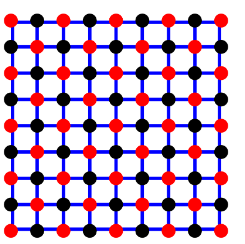
\includegraphics[width=0.3\textwidth]{figurest/figure_1.png} 
\end{figure}
\end{frame}








\begin{frame}
\begin{tabular}{l}
\hline
{\color{blue}算法2.4}求解二维离散poisson方程的红黑排序G-S迭代方法\\
\hline
1:Choose an initial guess $v^{(0)}$\\
2: while not converge do\\
3:\qquad for $(i,j)$为红色节点 do\\
4:\qquad \qquad
$u_{i, j}^{(k+1)}=\frac{1}{4}\left(h^{2} f_{i, j}+u_{i+1, j}^{(k)}+u_{i-1, j}^{(k)}+u_{i, j+1}^{(k)}+u_{i, j-1}^{(k)}\right)$\\
5:\qquad end for\\
6:\qquad for $(i,j)$为黑色节点 do\\
7:\qquad \qquad
$u_{i, j}^{(k+1)}=\frac{1}{4}\left(h^{2} f_{i, j}+u_{i+1, j}^{(k+1)}+u_{i-1, j}^{(k+1)}+u_{i, j+1}^{(k+1)}+u_{i, j-1}^{(k+1)}\right)$\\
8:\qquad end for\\
9:end while\\
\hline
\end{tabular}\\
\end{frame}

\begin{frame}
{SOR迭代}
在G-S算法的基础上,我们可以通过引入一个松弛参数$\omega$来加快收敛速度.这就是SOR (Successive Overrelaxation)算法,即将G-S算法中的第$k+1$步近似解与第k步近似解做一个加权平均:
\begin{align}
x^{(k+1)}=(1-\omega) x^{(k)}+\omega\left(D^{-1}\left(L x^{(k+1)}+U x^{(k)}\right)+D^{-1} b\right)\tag{6.10}
\end{align}
整理后即为
\begin{align}
x^{(k+1)}=(D-\omega L)^{-1}((1-\omega) D+\omega U) x^{(k)}+\omega(D-\omega L)^{-1} b\tag{6.11}
\end{align}
其中$\omega$称为{\color{blue}松弛参数}。\\
当$\omega=1$时,SOR即为G-S算法,当$\omega<$时,称为{\color{blue}低松弛(under relaxation)}算法,当$\omega>1$时,称为{\color{blue}超松弛(over relaxation)}算法.\\
\end{frame}

\begin{frame}
SOR算法曾经在很长一段时间内是科学计算中求解线性方程组的首选方法。在大多数情况下,当$\omega>1$时会取得比较好的收敛效果.\\
SOR的迭代矩阵为
$$
G_{\mathrm{SOR}}=(D-\omega L)^{-1}((1-\omega) D+\omega U)
$$

对应的矩阵分裂为
$$
M=\frac{1}{\omega} D-L, \quad N=\frac{1-\omega}{\omega} D+U
$$
由({\color{blue}6.11})可得SOR迭代的分量形式为
$$
\begin{aligned} x_{i}^{(k+1)} &=(1-\omega) x_{i}^{(k)}+\frac{\omega}{a_{i i}}\left(b_{i}-\sum_{j=1}^{i-1} a_{i j} x_{j}^{(k+1)}-\sum_{j=i+1}^{n} a_{i j} x_{j}^{(k)}\right) \\ &=x_{i}^{(k)}+\frac{\omega}{a_{i i}}\left(b_{i}-\sum_{j=1}^{i-1} a_{i j} x_{j}^{(k+1)}-\sum_{j=i}^{n} a_{i j} x_{j}^{(k)}\right) \end{aligned}
$$
\end{frame}

\begin{frame}
\begin{tabular}{l}
\hline
{\color{blue}算法2.5}求解线性方程组的SOR迭代方法\\
\hline
1:Choose an initial guess $x^{(0)}$\\
2: while not converge do\\
3:\qquad for $i=1$ to n do\\
4:\qquad \qquad
$x_{i}^{(k+1)}=(1-\omega) x_{i}^{(k)}+\frac{\omega}{a_{i i}}\left(b_{i}-\sum_{j=1}^{i-1} a_{i j} x_{j}^{(k+1)}-\sum_{j=i+1}^{n} a_{i j} x_{j}^{(k)}\right)$\\
5:\qquad end for\\
6:end while\\
\hline
\end{tabular}\\
SOR算法最大的优点是引入了松弛参数$\omega$,通过选取适当的$\omega$可以大大提高算法的收敛速度.\\
但是SOR算法最大的难点就是如何选取最优的参数\\
\end{frame}

\begin{frame}
\begin{tabular}{l}
\hline
{\color{blue}算法2.6}求解二维离散poisson方程的红黑排序G-S迭代方法\\
\hline
1:Choose an initial guess $v^{(0)}$\\
2: while not converge do\\
3:\qquad for $(i,j)$为红色节点 do\\
4:\qquad \qquad
$u_{i, j}^{(k+1)}=(1-\omega) v_{i, j}^{(k)}+\omega\left(h^{2} f_{i, j}+u_{i+1, j}^{(k)}+u_{i-1, j}^{(k)}+u_{i, j+1}^{(k)}+\right.$
$u_{i, j-1}^{(k)} ) / 4$\\
5:\qquad end for\\
6:\qquad for $(i,j)$为黑色节点 do\\
7:\qquad \qquad
$u_{i, j}^{(k+1)}=(1-\omega) v_{i, j}^{(k)}+\omega\left(h^{2} f_{i, j}+u_{i+1, j}^{(k+1)}+u_{i-1, j}^{(k+1)}+u_{i, j+1}^{(k+1)}+\right.$
$u_{i, j-1}^{(k+1)} ) / 4$\\
8:\qquad end for\\
9:end while\\
\hline
\end{tabular}\\
\end{frame}


\begin{frame}
{SSOR迭代方法}
将SOR算法中的L和U相交换,即可得迭代格式
$$
x^{(k+1)}=(D-\omega U)^{-1}((1-\omega) D+\omega L) x^{(k)}+\omega(D-\omega U)^{-1} b
$$
将这个迭代格式与SOR相结合,就可以得到下面的两步迭代方法
$$
\left\{\begin{array}{l}{x^{\left(k+\frac{1}{2}\right)}=(D-\omega L)^{-1}[(1-\omega) D+\omega U] x^{(k)}+\omega(D-\omega L)^{-1} b} \\ {x^{(k+1)}=(D-\omega U)^{-1}[(1-\omega) D+\omega L] x^{\left(k+\frac{1}{2}\right)}+\omega(D-\omega U)^{-1} b}\end{array}\right.
$$
这就是{\color{blue}SSOR迭代}(对称超松弛)算法,相当于将L与U同等看待,交替做两次SOR迭代.\\
消去中间迭代量$x^{(k+\frac{1}{2})}$,可得
$$
x^{(k+1)}=G_{\mathrm{SSOR}} x^{(k)}+g
$$
\end{frame}

\begin{frame}
其中迭代矩阵
$$
G_{\mathrm{SSOR}}=(D-\omega U)^{-1}[(1-\omega) D+\omega L](D-\omega L)^{-1}[(1-\omega) D+\omega U]
$$
对应的矩阵分裂为
$$
\begin{aligned} M &=\frac{1}{\omega(2-\omega)}\left[D-\omega(L+U)+\omega^{2} L D^{-1} U\right] \\ &=\frac{1}{\omega(2-\omega)}(D-\omega L) D^{-1}(D-\omega U) \\ N &=\frac{1}{\omega(2-\omega)}[(1-\omega) D+\omega L] D^{-1}[(1-\omega) D+\omega U] \end{aligned}
$$
对于某些特殊问题, SOR算法不收敛,但仍然可能构造出收敛的SSOR算法.\\
一般来说, SOR算法的渐进收敛速度对参数$\omega$比较敏感,但SSOR对参数$\omega$不太敏感.\\
({\color{blue} Poisson SOR omega.m,Poisson SSOR omega.m)})\\
\end{frame}


\begin{frame}
{AOR迭代}
Hadjidimos于1978年提出了AOR (Accelerated over-relaxation,快速松弛)算法,迭代矩阵为
$$
G_{\mathrm{AOR}}=(D-\gamma L)^{-1}[(1-\omega) D+(\omega-\gamma) L+\omega U]
$$
其中$\gamma$和$\omega$为松弛参数.对应的矩阵分解为
$$
M=\frac{1}{\omega}(D-\gamma L), \quad N=\frac{1}{\omega}[(1-\omega) D+(\omega-\gamma) L+\omega U]
$$
\begin{tabular}{l}
\qquad  (1)当$\gamma=\omega$时, AOR算法即为SOR算法;\\
\qquad  (2)当$\gamma=\omega=1$时, AOR算法即为G-S算法;\\
\qquad  (3)当$\gamma=0,\omega=1$时, AOR算法即为Jacobi算法
\end{tabular}
与SSOR类似,我们也可以定义SAOR算法.
\end{frame}

\begin{frame}{Richardson算法}
Richardson算法是一类形式非常简单的算法,其迭代格式为
$$
x^{(k+1)}=x^{(k)}+\omega\left(b-A x^{(k)}\right), \quad k=0,1,2, \ldots
$$
对应的矩阵分裂和迭代矩阵分别为
$$
M=\frac{1}{\omega} I, \quad N=\frac{1}{\omega} I-A, \quad G_{\mathrm{R}}=I-\omega A
$$
如果在每次迭代时取不同的参数,即
$$
x^{(k+1)}=x^{(k)}+\omega_{k}\left(b-A x^{(k)}\right), \quad k=0,1,2, \ldots
$$
则称为nonstationary Richardson算法.
\end{frame}

\begin{theorem}
设$A \in \mathbb{R}^{n \times n}$是对称正定矩阵,$\lambda_1$和$\lambda_n$分别是$A$的最大和最小特征值,则Richardson算法收敛当且仅当
$$
0<\omega<\frac{1}{\lambda_{1}}
$$
最优参数为
$$
\omega_{*}=\arg \min _{\omega} \rho\left(G_{\mathrm{R}}\right)=\frac{2}{\lambda_{1}+\lambda_{n}}
$$
即当$\omega=\omega_{*}$时,迭代矩阵的谱半径达到最小,且有
$$
\rho\left(G_{\mathrm{R}}\right)=\left\{\begin{array}{ll}{1-\omega \lambda_{n}} & {\text { if } \omega \leq \omega} \\ {\frac{\lambda_{1}-\lambda_{n}}{\lambda_{1}+\lambda_{n}}=\frac{\kappa(A)-1}{\kappa(A)+1}} & {\text { if } \omega=\omega} \\ {\omega \lambda_{1}-1} & {\text { if } \omega \geq \omega}\end{array}\right.
$$
\end{theorem}

\begin{frame}
{分块迭代方法}
前面介绍的迭代方法可以推广到分块情形.将$A$写成如下的分块形式
$$
A=\left[\begin{array}{cccc}{A_{11}} & {A_{12}} & {\cdots} & {A_{1 p}} \\ {A_{21}} & {A_{22}} & {\cdots} & {A_{2 p}} \\ {\vdots} & {\vdots} & {\ddots} & {\vdots} \\ {A_{p 1}} & {A_{p 2}} & {\cdots} & {A_{P P}}\end{array}\right]
$$
设$A=D-L-U$,其中$D,-L,-U$分别是A的快对角,块严格下三角矩阵和块严格上三角矩阵。则相应的分块Jacobi,分块Gauss-Seidel和分块SOR算法分别为
\begin{figure}[h]
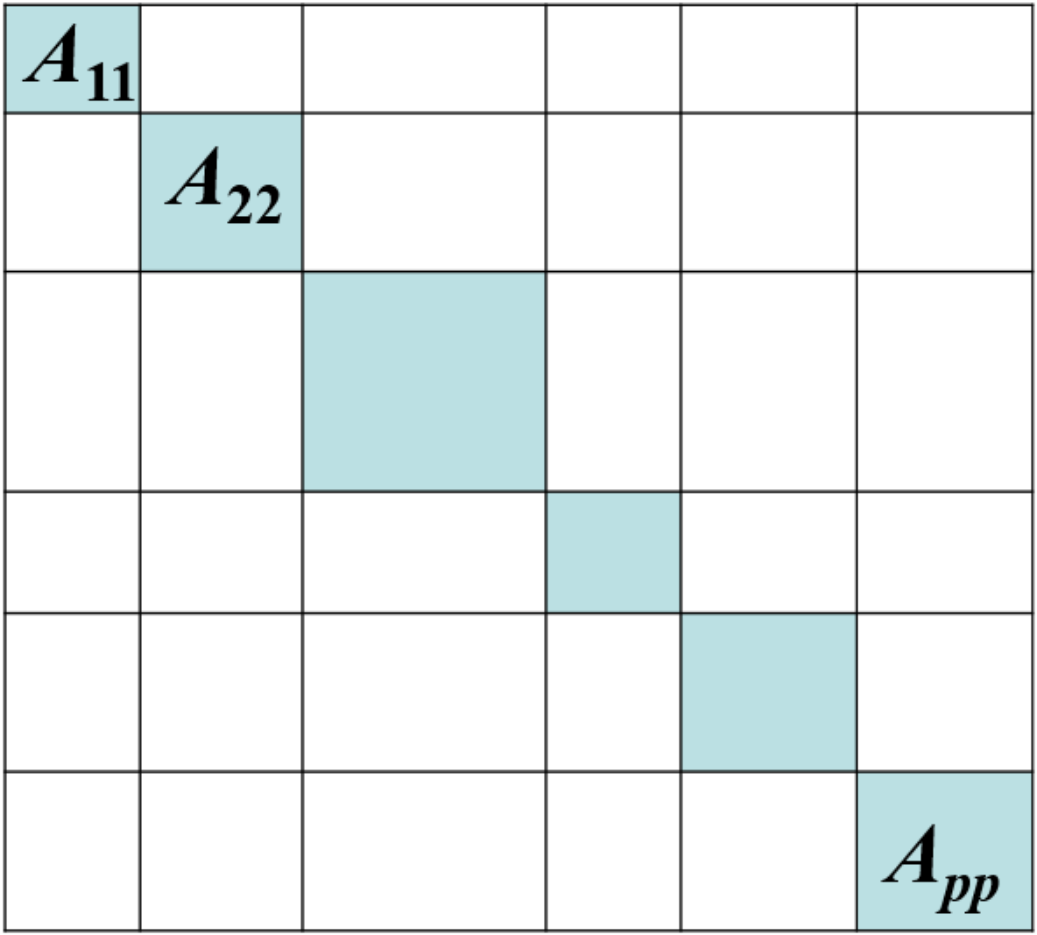
\includegraphics[width=0.3\textwidth]{figurest/figure_2.png} 
\end{figure}
\end{frame}

\begin{frame}
\begin{itemize}
\item {\color{blue}分块Jacobi迭代}
$$
A_{i i} \boldsymbol{x}_{i}^{(k+1)}=\boldsymbol{b}_{i}-\sum_{j=1, j \neq i}^{p} A_{i j} \boldsymbol{x}_{j}^{(k)}, \quad i=1,2, \ldots, p
$$
\item {\color{blue}分块Gauss-seidel迭代}$$
A_{i i} \boldsymbol{x}_{i}^{(k+1)}=\boldsymbol{b}_{i}-\sum_{j=1}^{i-1} A_{i j} \boldsymbol{x}_{j}^{(k+1)}-\sum_{j=i+1}^{p} A_{i j} \boldsymbol{x}_{j}^{(k)}, \quad i=1,2, \ldots, p
$$
\item {\color{blue}分块SOR迭代}$$
\begin{array}{c}{\boldsymbol{x}_{i}^{(k+1)}=(1-\omega) \boldsymbol{x}_{i}^{(k)}+\omega A_{i i}^{-1}\left(\boldsymbol{b}_{i}-\sum_{j=1}^{i-1} A_{i j} \boldsymbol{x}_{j}^{(k+1)}-\sum_{j=i+1}^{p} A_{i j} \boldsymbol{x}_{j}^{(k)}\right)} \\ {i=1,2, \ldots, p}\end{array}
$$
\end{itemize}
\end{frame}

\section{收敛性分析}

\begin{frame}
{定常迭代方法的收敛性}


{\color{blue}定义(迭代方法的收敛性)}如果对于任意的初始向量$x^{(0)}$,都有
$$\lim_{k\to \infty}x^{(k)}\to x_*$$
则称迭代格式{\color{blue}6.7}是{\color{blue}收敛}的,否则就称其为{\color{blue}发散}的。

基于矩阵分裂的迭代方法,其收敛性取决于迭代矩阵的谱半径.
\end{frame}

\begin{frame}


{\color{blue}\Large 矩阵谱半径}

\quad

\normalsize
设$A \in \mathbb{R}^{n \times n}$,则称
$$
\rho(A) \triangleq \max _{\lambda \in \sigma(A)}|\lambda|
$$
为$A$的{\color{blue}谱半径},其中$\sigma(A)$表示$A$的所有特征值组成的集合。\\
谱半径与矩阵范数之间有如下的关系.\\

\begin{lemma}[谱半径与范数的关系]
设$G \in \mathbb{R}^{n \times n}$,则
\begin{itemize}
\item[(1)]对任意算子范数,有$\rho(G) \leq\|G\|$;
\item[(2)]反之,对任意$\varepsilon>0$,都存在一个算子范数$\|\cdot\|_{\varepsilon}$,使得$| G \|_{\varepsilon} \leq\rho(G)+\varepsilon$,其中范数$\|\cdot\|_{\varepsilon}$依赖于$G$和$\varepsilon$.所以,若$\rho(G)<1$,则存在算子范数$\|\cdot\| \varepsilon$,使得$| G \|_{\varepsilon}<1$;
\end{itemize}
\end{lemma}
\end{frame}

\begin{frame}
由此,我们可以立即得到下面的结论.\\
\begin{definition}
设矩阵$G \in \mathbb{R}^{n \times n}$,则$\lim _{k \rightarrow \infty} G^{k}=0$当且仅当$\rho(G)<1$.
下面的结论是谱半径与算子范数之间的一个非常重要的性质。\\
\end{definition}

\begin{lemma}
设$G \in \mathbb{R}^{n \times n}$,则对任意算子范数$\|\cdot\|$,有
$$
\rho(G)=\lim _{k \rightarrow \infty}\left\|G^{k}\right\|^{\frac{1}{k}}
$$
\end{lemma}
\end{frame}

\begin{frame}

{\color{blue}\Large 迭代方法收敛性判断}

\quad

\normalsize
首先给出一个迭代方法收敛的充分条件\\
\begin{lemma}
若存在算子范数$\|\cdot\|$,使得$| G \|<1$,则迭代方法6.7收敛.\\
\end{lemma}
我们记$e^{(k)} \triangleq x^{(k)}-x$为第$k$步迭代解$x^{(k)}$的{\color{blue}误差向量}.\\
\begin{theorem}[收敛性定理]
对任意迭代初始向量$x^{(0)}$,迭代方法6.7收敛的充要条件是$\rho(G)<1$.\\
\end{theorem}

\end{frame}

\begin{frame}
\begin{definition}
设$G$是迭代矩阵,则迭代方法6.7的{\color{blue}平均收敛速度}定义为
$$
R_{k}(G) \triangleq-\ln \left\|G^{k}\right\|^{\frac{1}{k}}
$$,
{\color{blue}渐进收敛速度}定义为
$$
R(G) \triangleq \lim _{k \rightarrow \infty} R_{k}(G)=-\ln \rho(G)
$$
\end{definition}
平均收敛速度与迭代步数和所用的范数有关,但渐进收敛速度只依赖于迭代矩阵的谱半径.\\
\end{frame}

\begin{theorem}
考虑算法6.7.如果存在某个算子范数$\|\cdot\|$使得$\|G\|=q<1$,则
\begin{itemize}
\item[(1)]$\left\|x^{(k)}-x_{*}\right\| \leq q^{k}\left\|x^{(0)}-x_{*}\right\|$

\item[(2)]$\left\|x^{(k)}-x_{+}\right\| \leq \frac{q}{1-q}\left\|x^{(k)}-x^{(k-1)}\right\|$

\item[(3)]$\left\|x^{(k)}-x_{*}\right\| \leq \frac{q^{k}}{1-q}\left\|x^{(1)}-x^{(0)}\right\|$
\end{itemize}
\end{theorem}

一般来说,好的迭代方法应该满足
\begin{itemize}
\item[(1)]$\rho(G)$很小

\item[(2)]以$M$为系数矩阵的线性方程组比较容易求解;
\end{itemize}

\begin{frame}
{二维离散Poisson方程情形}


{\color{blue}充要条件}:迭代矩阵的谱半径小于1.\\
{\color{blue}充分条件}:迭代矩阵的某个算子范数小于1.\\
对于二维离散Poisson方程,系数矩阵为
$$
A=T=I \otimes T_{n}+T_{n} \otimes I
$$
故Jacobi算法的迭代矩阵为

\begin{align*}
G_{\mathrm{J}}=D^{-1}(L+U)=(4 I)^{-1}(4 I-T)=I-\frac{1}{4} T
\tag {6.12}
\end{align*}

由于$T$的特征值为
$$
\lambda_{i}+\lambda_{j}=2\left(1-\cos \frac{\pi i}{n+1}\right)+2\left(1-\cos \frac{\pi j}{n+1}\right)
$$
\end{frame}

\begin{frame}
所以$G_{\mathrm{J}}$的特征值为
$$
1-\frac{1}{4}\left(\lambda_{i}+\lambda_{j}\right)=\frac{1}{2}\left(\cos \frac{\pi i}{n+1}+\cos \frac{\pi j}{n+1}\right)
$$
故
$$
\rho\left(G_{\mathrm{J}}\right)=\frac{1}{2} \max _{i, j}\left\{\left|\cos \frac{\pi i}{n+1}+\cos \frac{\pi j}{n+1}\right|\right\}=\cos \frac{\pi}{n+1}<1
$$
即Jacobi算法是收敛的.

注意当$n$越来越大时,$\kappa(T) \rightarrow \infty$,即$T$越来越病态,此时$\rho\left(G_{1}\right) \rightarrow 1$,即Jacobi算法收敛越来越慢.\\
{\color{blue}问题越病态可能就越难求解}
\end{frame}

\begin{frame}


{\color{blue}\Large G-S算法和SOR算法}

\quad

\normalsize
{\color{blue}性质}设$G_{\mathrm{GS}}$和$G_{\mathrm{SOR}}$分别表示求解二维Poisson方程的红黑排序的G-S算法和SOR算法的迭代矩阵,则有
\begin{align*}
\rho\left(G_{\mathrm{GS}}\right)=\rho\left(G_{\mathrm{J}}\right)^{2}=\cos ^{2} \frac{\pi}{n+1}<1
\tag{6.13}
\end{align*}
\begin{align*}
\rho\left(G_{\mathrm{SOR}}\right)=\frac{\cos ^{2} \frac{\pi}{n+1}}{\left(1+\sin \frac{\pi}{n+1}\right)^{2}}<1, \quad \omega=\frac{2}{1+\sin \frac{\pi}{n+1}}
\tag{6.14}
\end{align*}
在上述结论中, SOR算法中的$\omega$是最优参数,即此时的$\rho\left(G_{\mathrm{SOR}}\right)$最小.
\end{frame}


\begin{frame}


{\color{blue}\Large SOR与Jacobi}

\quad

\normalsize
由Taylor公式可知,当$n$很大时,有
$$
\begin{aligned} \rho\left(G_{\mathrm{J}}\right) &=\cos \frac{\pi}{n+1} \approx 1-\frac{\pi^{2}}{2(n+1)^{2}}=1-O\left(\frac{1}{n^{2}}\right) \\ \rho\left(G_{\mathrm{SOR}}\right) &=\frac{\cos ^{2} \frac{\pi}{n+1}}{\left(1+\sin \frac{\pi}{n+1}\right)^{2}} \approx 1-\frac{2 \pi}{n+1}=1-O\left(\frac{1}{n}\right) \end{aligned}
$$
由于当$n$很大时有
$$
\left(1-\frac{1}{n}\right)^{k} \approx 1-\frac{k}{n}=1-\frac{k n}{n^{2}} \approx\left(1-\frac{1}{n^{2}}\right)^{k n}
$$
即SOR迭代$k$步后误差的减小量与Jacobi迭代$kn$步后误差减小量差不多.因此,取最优参数的$SOR$算法的收敛速度大约是$Jacobi$算法的$n$倍.\\
\end{frame}

\begin{frame}
事实上,当$n$很大时,这三个算法的收敛速度都很慢.\\
{\color{blue}例}\quad 已知二维Poisson方程
$$
\left\{\begin{array}{ll}
{-\Delta u(x, y)=-1,} & {(x, y) \in \Omega} \\ 
{u(x, y)=\frac{x^{2}+y^{2}}{4},} & {(x, y) \in \partial \Omega}\end{array}\right.
$$
其中$\Omega=(0,1) \times(0,1)$.该方程的解析解是$u(x, y)=\frac{x^{2}+y^{2}}{4}$.用五点差分格式离散后得到一个线性方程组,分别用Jacobi, G-S和SOR算法计算这个方程组的解,并比较收敛效果
\end{frame}

\begin{figure}[h]
\centering 
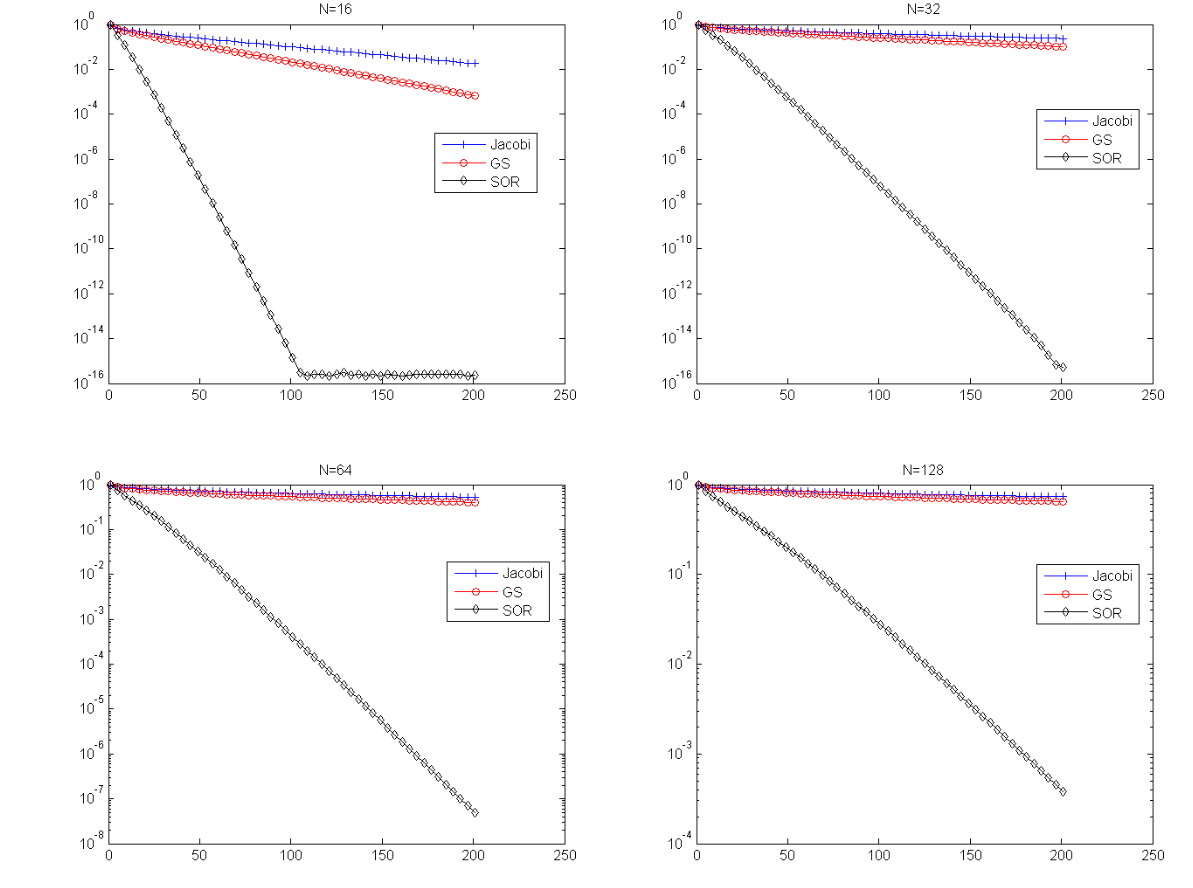
\includegraphics[width=1\textwidth]{figurest/figure_3.png} 
\end{figure}

\begin{frame}
{不可约对角占优}
这里我们考虑A是严格对角占优或不可约弱对角占优情形.
\begin{theorem}
设$A \in \mathbb{R}^{n \times n}$,若A严格对角占优,则Jacobi算法和G-S算法都收敛,且
$$
\left\|G_{\mathrm{GS}}\right\|_{\infty} \leq\left\|G_{\mathrm{J}}\right\|_{\infty}<1
$$
\end{theorem}
\end{frame}

\begin{frame}
\begin{theorem}
设$A \in \mathbb{R}^{n \times n}$若A是弱对角占优且不可约,则Jacobi算法和G-S算法都收敛,且$\rho\left(G_{\mathrm{GS}}\right)<\rho\left(G_{\mathrm{J}}\right)<1$
\end{theorem}

二维离散Poisson方程是弱行对角占优且不可约,故对Jacobi算法和G-S算法都收敛.

上述定理中的结论对一般矩阵并不成立:{\color{blue}对某些矩阵, Jacobi算法收敛,但G-S算法却不一定收敛}.
\end{frame}

\begin{frame}
关于SOR方法,我们有下面的结论

设$A \in \mathbb{R}^{n \times n}$,若A严格对角占优且$0<\omega \leq 1$,则SOR方法收敛.\\
{\color{blue}定理}\quad 设$A \in \mathbb{R}^{n \times n}$若A是弱对角占优且不可约,且$0<\omega \leq 1$则SOR方法收敛.
\end{frame}

\begin{frame}
{对称正定矩阵}
在给出收敛性结论之前,也介绍两个需要用到的引理.\\
{\color{blue}引理}\quad 设$A \in \mathbb{C}^{n \times n}$,Hermite对称,且$A=M-N$是$A$的一个矩阵分裂,则$M^{*}+N$也是Hermite对称,且对任意$x \in \mathbb{C}^{n}$有
$$
x^{*} A x-\tilde{x}^{*} A \tilde{x}=u^{*}\left(M^{*}+N\right) u
$$
其中$\tilde{x}=M^{-1} N x, u=x-\tilde{x}$
{\color{blue}定理}\quad 设$A \in \mathbb{R}^{n \times n}$对称,且$A=M-N$是$A$的一个矩阵分裂.
\begin{itemize}
\item[(1)]如果$A$和$M^{T}+N$都是正定矩阵,则$M$非奇异且$\rho\left(M^{-1} N\right)<1$

\item[(2)]如果$\rho\left(M^{-1} N\right)<1$且$M^{T}+N$正定,则$A$正定.
\end{itemize}
\end{frame}

\begin{frame}
我们首先给出SOR迭代收敛的一个必要条件.
{\color{blue}定理}对于SOR算法,有$\rho\left(G_{\mathrm{SOR}}\right) \geq|1-\omega|$,故SOR算法收敛的必要条件是$0<\omega<2$.
{\color{blue}定理}\quad 设$A \in \mathbb{R}^{n \times n}$对称正定.
\begin{itemize}
\item[(1)]若$2D$正定且Jacobi迭代收敛,则$A$正定

\item[(2)]若$D$正定,且存在$\omega \in(0,2)$使得SOR (或SSOR)收敛,则$A$正定

\item[(3)]若$D$正定,且G-S迭代收敛,则$A$正定.
\end{itemize}
\end{frame}


\begin{frame}{相容次序矩阵}
针对一类特殊的矩阵,这三种迭代方法的谱半径之间存在一种特殊关系.\\
{\color{blue}定义}设$A \in \mathbb{R}^{n \times n}$,如果存在一个置换矩阵$P$,使得
\begin{align}
P A P^{T}=\left[\begin{array}{cc}{D_{1}} & {F} \\ {E} & {D_{2}}\end{array}\right]\tag{6.15}
\end{align}
其中$D_{1}, D_{2}$为对角矩阵,则称$A$具有{\color{blue}性质A}.
{\color{blue}例}\quad 对于二维离散Poisson方程,系数矩阵$T_{N^{2}}$具有性质$A$.事实上,设$\tilde{T}_{N^{2}}$为模型问题采用红黑排序后的系数矩阵,则$\tilde{T}_{N^{2}}$具有({\color{blue}6.15})的结构.\\
\end{frame}

\begin{frame}
我们首先给出一个性质.\\
\begin{lemma}
\quad 设$B \in \mathbb{R}^{n \times n}$具有下面的结构
$$
B=\left[\begin{array}{cc}{0} & {B_{12}} \\ {B_{21}} & {0}\end{array}\right]
$$
令$B_L$和$B_U$分别表示$B$的下三角和上三角部分,则
\begin{itemize}
\item[(1)]若$\mu$是$B$的特征值,则$-\mu$也是$B$的特征值;

\item[(2)]$B(\alpha)$的特征值与无关,其中
$$
B(\alpha)=\alpha B_L+\frac{1}{\alpha}B_U,\qquad \alpha \ne 0
$$
\end{itemize}
\end{lemma}

$B(\alpha)+\beta I$的特征值也与$\alpha$无关,其中$\beta$为任意常数.
\end{frame}

\begin{frame}
该结论可以推广到块三对角形式,见习题.
设$A \in \mathbb{R}^{n \times n}$的对角线元素全不为零,记$\tilde{L}=D^{-1} L, \tilde{U}=D^{-1} U$.

\begin{definition}
设$A \in \mathbb{R}^{n \times n}$的对角线元素全不为零,$A=D(I-\tilde{L}-\tilde{U})$若矩阵$G(\alpha)=\alpha \tilde{L}+\frac{1}{\alpha} \tilde{U}$的特征值与$\alpha$无关,则称$A$具有相容次序.\\
\end{definition}

设$A$的对角线元素全不为零,若$A$具有性质$A$,则存在置换矩阵$P$,使得$P A P^{T}$具有相容次序.\\

\end{frame}

\begin{frame}
\begin{theorem}
设$A$有相容次序且$\omega \neq 0$,则下列命题成立

(1)Jacobi迭代矩阵$G_{\mathrm{l}}$的特征值正负成对出现;

(2)若$\mu$是$G_{\mathrm{J}}$的特征值且$\lambda$满足
\begin{align}
	(\lambda+\omega-1)^{2}=\lambda \omega^{2} \mu^{2}\tag{6.16}
\end{align}
则$\lambda$是$SOR$迭代矩阵$G_{\mathrm{SOR}}$的一个特征值;

(3)反之,若$\lambda \neq 0$是$G_{\mathrm{SOR}}$的一个特征值且$\mu$满足(6.16),则$\mu$是$G_{\mathrm{J}}$的一个特征值.

\end{theorem}

{\color{blue}推论}\quad 若$A$具有相容次序,则$\rho\left(G_{\mathrm{GS}}\right)=\rho\left(G_{\mathrm{J}}\right)^{2}$,即当Jacobi算法收敛时,G-S算法比Jacobi算法快一倍
\end{frame}

\begin{frame}
{\color{blue}例}\qquad 采用红黑排序的二维离散Poisson方程,系数矩阵$\tilde{T}_{N^{2}}$具有相容次序,故有$\rho\left(G_{\mathrm{GS}}\right)=\rho\left(G_{\mathrm{J}}\right)^{2}$.
\end{frame}

\begin{frame}
下面是关于SOR算法的最优参数选取.
\begin{theorem}
设$A$具有相容次序,$G_{\mathrm{l}}$的特征值全部为实数,且$\rho_{J}=\rho\left(G_{\mathrm{J}}\right)<1$,则SOR算法的最优参数为
$$
\omega_{o p t}=\frac{2}{1+\sqrt{1-\rho_{J}^{2}}}
$$
此时
$$
\rho\left(G_{\mathrm{SOR}}\right)=\omega_{o p t}-1=\frac{\rho_{J}^{2}}{\left(1+\sqrt{1-\rho_{J}^{2}}\right)^{2}}
$$
进一步,有
$$
\rho\left(G_{\mathrm{SOR}}\right)=\left\{\begin{array}{ll}{\omega-1,} & {\omega_{o p t} \leq \omega \leq 2} \\ {1-\omega+\frac{1}{2} \omega^{2} \rho_{J}^{2}+\omega \rho_{J} \sqrt{1-\omega+\frac{1}{4} \omega^{2} \rho_{J}^{2}},} & {0<\omega \leq \omega_{o p t}}\end{array}\right.
$$
\end{theorem}
\end{frame}

\begin{frame}
{\color{blue}例}\qquad 采用红黑排序的二维离散Poisson问题的系数矩阵$\tilde{T}_{N^{2}}$具有相容次序,且$G_{\mathrm{l}}$是对称的,即$G_{\mathrm{l}}$的特征值都是实的.又由系数矩阵的弱对角占优和不可约性质可知$\rho\left(G_{1}\right)<1$,故上述定理的条件均满足.
\end{frame}

\section{加速算法}
\begin{frame}
当迭代解$x^{(0)}, x^{(1)}, x^{(2)}, \ldots, x^{(k)}$已经计算出来后,我们可以对其进行组合,得到一个新的近似解,这样就可以对原算法进行加速
\end{frame}

\begin{frame}
{外推技术}
设原迭代格式为
\begin{align*}
x^{(k+1)}=G x^{(k)}+b
\tag{6.17}
\end{align*}
由$x^{(k)}$和$x^{(k+1)}$加权组合后可得新的近似解
\begin{align*}
x^{(k+1)}=(1-\omega) x^{(k)}+\omega\left(G x^{(k)}+b\right)
\tag{6.18}
\end{align*}
其中$\omega$是参数.这种加速方法就称为{\color{blue}外推算法}.\\
为了使得迭代格式(6.18)尽可能快地收敛,需要选择$\omega$使得其迭代矩阵$G_{\omega} \triangleq(1-\omega) I+\omega G$的谱半径尽可能地小.假设$G$的特征值都是实数,且最大特征值和最小特征值分别为$\lambda_{1}$和$\lambda_{n}$.于是
$$
\rho\left(G_{\omega}\right)=\max _{\lambda \in \sigma(G)}|(1-\omega)+\omega \lambda|=\max \left\{\left|1-\omega+\omega \lambda_{1}\right|,\left|1-\omega+\omega \lambda_{n}\right|\right\}
$$
\end{frame}

\begin{frame}
\begin{definition}
设$G$的特征值都是实数,其最大和最小特征值分别为$\lambda_{1}$和$\lambda_{n}$,且1$\notin\left[\lambda_{n}, \lambda_{1}\right]$,则
$$
\omega_{*}=\arg \min _{\omega} \rho\left(G_{\omega}\right)=\frac{2}{2-\left(\lambda_{1}+\lambda_{n}\right)}
$$
此时
$$
\rho\left(G_{\omega_{*}}\right)=1-\left|\omega_{*}\right| d
$$
其中$d$是$1$到$\left[\lambda_{n}, \lambda_{1}\right]$的距离,即当$\lambda_{n} \leq \lambda_{1}<1$时,$d=\lambda_{n}-1$.\\
\end{definition}

由定理可知,$\rho\left(G_{\omega_{*}}\right)=1-\left|\omega_{*}\right| d$且当$\omega_{*} \neq 1$时,外推迭代(6.18)比原迭代方法收敛要更快一些.\\
最优参数依赖于原迭代矩阵$G$的特征值,因此实用性不强.在实际应用时可以估计特征值所在的区间$[a, b]$,然后用$a,b$代替$\lambda_{n}$和$\lambda_{1}$.
\end{frame}


\begin{frame}


{\color{blue}\Large JOR算法}

\quad

\normalsize
对$Jacobi$迭代进行外推加速,则可得$JOR (Jacobi over-relaxation)$算法:
$$
\begin{aligned} x^{(k+1)} &=(1-\omega) x^{(k)}+\omega\left(D^{-1}(L+U) x^{(k)}+D^{-1} b\right) \\ &=x^{(k)}+\omega D^{-1}\left(b-A x^{(k)}\right), \quad k=0,1,2, \ldots \end{aligned}
$$
\begin{theorem}
设$A$对称正定.若
$$
0<\omega<\frac{2}{\rho\left(D^{-1} A\right)}
$$
则JOR算法收敛.
\end{theorem}

\end{frame}

\begin{frame}
{Chebyshev加速}
本节对外推技巧进行推广.\\
假定通过迭代格式(6.17)已经计算出$x^{(0)}, x^{(1)}, \ldots, x^{(k)}$,下面考虑如何将这些近似解进行组合,以便得到更精确的近似解.\\
记$\varepsilon_{k}=x^{(k)}-x_{*}$为第$k$步迭代解的误差,则有
$$
\varepsilon_{k}=G \varepsilon_{k-1}=G^{2} \varepsilon_{k-2}=\cdots=G^{k} \varepsilon_{0}
$$
设$\tilde{x}^{(k)}$为$x^{(0)}, x^{(1)}, \ldots, x^{(k)}$的一个线性组合,即
\begin{align*}
\tilde{x}^{(k)}=\alpha_{0} x^{(0)}+\alpha_{1} x^{(1)}+\cdots+\alpha_{k} x^{(k)}
\tag{6.19}
\end{align*}
其中$\alpha_{i}$为待定系数,且满足$\sum_{i=0}^{k} \alpha_{i}=1$.于是
\begin{align*}
\tilde{x}^{(k)}-x_{*}=\alpha_{0} \varepsilon_{0}+\alpha_{1} G \varepsilon_{0}+\cdots+\alpha_{k} G^{k} \varepsilon_{0} \triangleq p_{k}(G) \varepsilon_{0}
\tag{6.20}
\end{align*}
\end{frame}

\begin{frame}
其中$p_{k}(t)=\sum_{i=0}^{k} \alpha_{i} t^{i}$为$k$次多项式,且满足$p_{k}(1)=1$.\\
我们希望通过适当选取参数$\alpha_i$,使得$\tilde{x}^{(k)}-x_*$尽可能地小,即使得$\tilde{x}^{(k)}$收敛到$x_*$速度远远快于$x^{(k)}$收敛到$x$速度.这种加速方法就称为{\color{blue}多项式加速}或{\color{blue}半迭代方法(semi-iterative method)}\\
{\color{blue}例}\qquad 设$p_{n}(t)$为$G$的特征多项式,则$p_{n}(G)=0$,所以选取$\alpha_i$为$p_n$的系数,则$\tilde{x}^{(n)}-x_{*}=0$.但这种选取方法不实用,原因是:
\begin{itemize}
\item[(1)]$p_{n}(t)$的系数并不知道;

\item[(2)]我们通常希望收敛所需的迭代步数$\ll n$.
\end{itemize}

\end{frame}

\begin{frame}
下面讨论参数$\alpha_i$的较实用的选取方法.由(6.20)可知
$$\left\|\tilde{x}^{(k)}-x_{*}\right\|_{2}=\left\|p_{k}(G) \varepsilon_{0}\right\|_{2} \leq\left\|p_{k}(G)\right\|_{2} \cdot\left\|\varepsilon_{0}\right\|_{2}$$
因此我们需要求解下面的极小化问题
\begin{align*}
\min _{p \in \mathbb{P}_{k}, p(1)=1}\|p(G)\|_{2}
\tag{6.21}
\end{align*}
其中$\mathbb{P}_{k}$表示所有次数不超过k的多项式组成的集合.\\
一般来说,这个问题是非常困难的.\\
但在一些特殊情况下,我们可以给出其最优解.\\
\end{frame}

\begin{frame}
假设迭代矩阵$G$是对称的,即$G$存在特征值分解$Schur$标准型为
$$
G=U \Lambda U^{*}
$$
其中$\Lambda$是实对角矩阵,$U$是酉矩阵.于是有
\begin{align*}
\begin{array}{ll}
	\min _{p \in \mathbb{P}_{k, P}(1)=1}\|p(G)\|_{2}&{=\min _{p \in \mathbb{P}_{k, p}(1)=1}^{\min }\|p(\Lambda)\|_{2}} \\ {}&{=\min _{p \in \mathbb{P}_{k, p}(1)=1} \max _{1 \leq i \leq n}\left\{\left|p\left(\lambda_{i}\right)\right|\right\}} \\ {}&{ \leq \min _{p \in \mathbb{P}_{k, p}(1)=1} \max _{\lambda \in\left[\lambda_{n}, \lambda_{1}\right]}\{|p(\lambda)|\}}\end{array}
\tag{6.22}
\end{align*}
其中$\lambda_{1}, \lambda_{n}$分别表示$G$的最大和最小特征值.\\
这是带归一化条件的多项式最佳一致逼近问题(与零的偏差最小).\\
该问题的解与著名的{\color{blue}Chebyshev多项式}有关.\\
\end{frame}

\begin{frame}


{\color{blue}\Large Chebyshev多项式}

\quad

\normalsize
Chebyshev多项式$T_{k}(t)$可以通过下面的递归方式来定义:
\begin{align*}
\begin{array}{l}{T_{0}(t)=1, \quad T_{1}(t)=t} \\ {T_{k}(t)=2 t T_{k-1}(t)-T_{k-2}(t), k=2,3, \ldots}\end{array}
\tag{6.23}
\end{align*}
也可以直接由下面的式子定义
$$
T_{k}(t)=\frac{1}{2}\left[\left(t+\sqrt{t^{2}-1}\right)^{k}+\left(t+\sqrt{t^{2}-1}\right)^{-k}\right]
$$
或者
$$
T_{k}(t)=\left\{\begin{array}{ll}{\cos (k \text { arccost }),} & {|t| \leq 1} \\ {\cosh (k \operatorname{arccosh} t),} & {|t|>1}\end{array}\right.
$$
\end{frame}

\begin{frame}
Chebyshev的一个重要性质是下面的最小最大性质.\\
{\color{blue}定理}设$\eta \in \mathbb{R}$满足$|\eta|>1$,则下面的最小最大问题
$$
\min _{p(t) \in \mathbb{P}_{k}, p(\eta)=1-1 \leq t \leq 1}|p(t)|
$$
的唯一解为
$$
\tilde{T}_{k}(t) \triangleq \frac{T_{k}(t)}{T_{k}(\eta)}
$$
\end{frame}

\begin{frame}
通过简单的仿射变换,该定理的结论可以推广到一般区间.
{\color{blue}定理}\qquad 设$\alpha, \beta, \eta \in \mathbb{R}$满足$\alpha<\beta$且$|\eta| \notin[\alpha, \beta]$.则下面的最小最大问题
$$
\min _{p(t) \in \mathbb{P}_{k, p}(\eta)=1} \max _{\alpha \leq x \leq \beta}|p(t)|
$$
的唯一解为
$$
\hat{T}_{k}(t) \triangleq \frac{T_{k}\left(\frac{2 t-(\beta+\alpha)}{\beta-\alpha}\right)}{T_{k}\left(\frac{2 \eta-(\beta+\alpha)}{\beta-\alpha}\right)}
$$
\end{frame}

\begin{frame}


{\color{blue}\Large Chebyshev加速方法}

\quad

\normalsize
考虑迭代格式$x^(k+1)=Gx^(k)+b$,我们假定:
\begin{itemize}
\item[(1)]迭代矩阵$G$的特征值都是实数;
\item[(2)]迭代矩阵谱半径$\rho=\rho(G)<1$,故$\lambda(G) \in[-\rho, \rho] \subset(-1,1)$
\end{itemize}

于是最小最大问题(6.22)就转化为
$$
\min _{p \in \mathbb{P}_{k}, p(1)=1} \max _{\lambda \in[-\rho, \rho]}\{|p(\lambda)|\}
$$
由于$1 \neq[-\rho, \rho]$根据定理4.4,上述问题的解为
$$
p_{k}(t)=\frac{T_{k}(t / \rho)}{T_{k}(1 / \rho)}
$$
\end{frame}

\begin{frame}


{\color{blue}\Large $\tilde{x}^{(k)}$的计算}

\quad

\normalsize
我们无需先计算$x^{(0)}, x^{(1)}, \ldots, x^{(k)}$,然后通过线性组合(6.19)来计算$\tilde{x}^{(k)}$事实上,我们可以通过Chebyshev多项式的三项递推公式(6.23),由$\tilde{x}^{(k-1)}$和$\tilde{x}^{(k-2)}$直接计算出$\tilde{x}^{(k)}$.这样做的另一个好处是无需存储所有的$\tilde{x}^{(i)}$.具体的推导公式如下:\\
令$\mu_{k}=\frac{1}{T_{k}(1 / \rho)}$,即$T_{k}(1 / \rho)=\frac{1}{\mu_{k}}$.由三项递推公式(6.23)可得
$$
\frac{1}{\mu_{k}}=\frac{2}{\rho} \cdot \frac{1}{\mu_{k-1}}-\frac{1}{\mu_{k-2}}
$$
所以
$$
\begin{aligned} \tilde{x}^{(k)}-x_{*}=p_{k}(G) \varepsilon_{0} &=\mu_{k} T_{k}(G / \rho) \varepsilon_{0} \\ &=\mu_{k}\left[\frac{2 G}{\rho} \cdot \frac{1}{\mu_{k-1}}\left(\tilde{x}^{(k-1)}-x_{*}\right)-\frac{1}{\mu_{k-2}}\left(\tilde{x}^{(k-2)}-x_{*}\right)\right] \end{aligned}
$$
\end{frame}

\begin{frame}
整理后可得
$$
\boxed{\tilde{x}^{(k)}=\frac{2 \mu_{k}}{\mu_{k-1}} \cdot \frac{G}{\rho} \tilde{x}^{(k-1)}-\frac{\mu_{k}}{\mu_{k-2}} \tilde{x}^{(k-2)}+d_{k}}
$$
其中
$$
\begin{aligned} d_{k} &=x_{*}-\frac{2 \mu_{k}}{\mu_{k-1}} \cdot \frac{G}{\rho} x_{*}+\frac{\mu_{k}}{\mu_{k-2}} x_{*} \\ &=x^{*}-\frac{2 \mu_{k}}{\mu_{k-1}} \cdot \frac{x_{*}-g}{\rho}+\frac{\mu_{k}}{\mu_{k-2}} x_{*} \\ &=\mu_{k}\left(\frac{1}{\mu_{k}}-\frac{2}{\rho \mu_{k-1}}+\frac{1}{\mu_{k-2}}\right) x_{*}+\frac{2 \mu_{k} g}{\mu_{k-1} \rho} \\ &=\frac{2 \mu_{k} g}{\mu_{k-1} \rho} \end{aligned}
$$
\end{frame}

\begin{frame}
由此,我们可以得到迭代格式(6.17)的Chebyshev加速算法.\\
\begin{tabular}{l}
\hline
{\color{blue}算法4.1}Chebyshev加速算法\\
\hline
1:Set $\mu_{0}=1, \mu_{1}=\rho=\rho(G), \tilde{x}^{(0)}=x^{(0)}, k=1$\\
2:compute$\tilde{x}^{(1)}=G x^{(0)}+g$\\
3:while not converge do\\
4:\qquad$k=k+1$\\
5:\qquad$\mu_{k}=\left(\frac{2}{\rho} \cdot \frac{1}{\mu_{k-1}}-\frac{1}{\mu_{k-2}}\right)^{-1}$\\
6:\qquad$\tilde{x}^{(k)}=\frac{2 \mu_{k}}{\mu_{k-1}} \cdot \frac{G}{\rho} \tilde{x}^{(k-1)}-\frac{\mu_{k}}{\mu_{k-2}} \tilde{x}^{(k-2)}+\frac{2 \mu_{k}}{\mu_{k-1} \rho} \cdot g$\\
7:end while\\
\hline
\end{tabular}

该算法的每步迭代的整体运算量与原迭代格式基本相当.\\
设$\lambda(G) \in[\alpha, \beta]$,且$-1<\alpha \leq \beta<1$,则我们也可以构造出相应的Chebyshev加速算法.
\end{frame}

\begin{frame}


{\color{blue}\Large SSOR算法的Chebyshev加速}

\quad

\normalsize
SSOR迭代矩阵为
$$
G_{\mathrm{SSOR}}=(D-\omega U)^{-1}[(1-\omega) D+\omega L](D-\omega L)^{-1}[(1-\omega) D+\omega U]
$$
当$A$对称时,有$L=U^{T}$,故
$$
\begin{array}{l}{(D-\omega U) G_{\mathrm{SSOR}}(D-\omega U)^{-1}} \\ {=[(1-\omega) D+\omega L](D-\omega L)^{-1}\left[(1-\omega) D+\omega L^{T}\right]\left(D-\omega L^{T}\right)^{-1}} \\ {=\left[(2-\omega) D(D-\omega L)^{-1}-I\right]\left[(2-\omega) D\left(D-\omega L^{T}\right)^{-1}-I\right]} \\ {=I-(2-\omega) D\left[(D-\omega L)^{-1}+\left(D-\omega L^{T}\right)^{-1}\right]} \\ {\quad+(2-\omega)^{2} D(D-\omega L)^{-1} D\left(I-\omega L^{T}\right)^{-1}}\end{array}
$$
\end{frame}

\begin{frame}
假定$D$的对角线元素全是正的,则
$$
\begin{array}{l}{D^{-1 / 2}(D-\omega U) G_{\mathrm{SSOR}}(D-\omega U)^{-1} D^{1 / 2}} \\ {=I-(2-\omega) D^{-1 / 2}\left[(D-\omega L)^{-1}+\left(D-\omega L^{T}\right)^{-1}\right] D^{1 / 2}} \\ {\quad+(2-\omega)^{2} D^{-1 / 2}(D-\omega L)^{-1} D\left(I-\omega L^{T}\right)^{-1} D^{1 / 2}}\end{array}
$$
这是一个对称矩阵,故$G_{\text { SSOR }}$具有实特征值.所以我们可以对其实行Chebyshev加速.但我们需要估计$G_{\text { SSOR }}$的谱半径.
若存在矩阵$W$使得$W^{-1} A W$是对称矩阵,则称$A$是可对称化的,即$A$相似于一个对称矩阵.\\
\end{frame}

\section{交替方向与HSS算法}
\begin{frame}
{多步迭代法}
设$A=M_{1}-N_{1}=M_{2}-N_{2}$是$A$的两个矩阵分裂,则可以构造迭代格式
\begin{align*}
\left\{\begin{array}{l}{M_{1} x^{\left(k+\frac{1}{2}\right)}=N_{1} x^{(k)}+b,} \\ {M_{2} x^{(k+1)}=N_{2} x^{\left(k+\frac{1}{2}\right)}+b}\end{array} \quad k=0,1,2, \ldots\right.
\tag{6.24}
\end{align*}
这就是两步迭代方法,对应的分裂称为二重分裂.\\
易知,两步迭代格式(6.24)的迭代矩阵为
$$
G=M_{2}^{-1} N_{2} M_{1}^{-1} N_{1}
$$
因此,其收敛的充要条件是$\rho\left(M_{2}^{-1} N_{2} M_{1}^{-1} N_{1}\right)<1$.
类似地,我们可以推广到多步迭代方法.
\end{frame}

\begin{frame}
{交替方向法}

{\color{blue}交替方向(ADI)}本质上是一个两步迭代方法
设$A=A_{1}+A_{2}$,则ADI迭代格式为
\begin{align*}
\left\{\begin{array}{l}{\left(\alpha I+A_{1}\right) x^{\left(k+\frac{1}{2}\right)}=\left(\alpha I-A_{2}\right) x^{(k)}+b,} \\ {\left(\alpha I+A_{2}\right) x^{(k+1)}=\left(\alpha I-A_{1}\right) x^{\left(k+\frac{1}{2}\right)}+b,}\end{array} \quad k=0,1,2, \ldots\right.
\tag{6.25}
\end{align*}
其中$\alpha \in \mathbb{R}$是迭代参数.易知ADI算法的迭代矩阵为
$$
G_{\mathrm{ADI}}=\left(\alpha I+A_{2}\right)^{-1}\left(\alpha I-A_{1}\right)\left(\alpha I+A_{1}\right)^{-1}\left(\alpha I-A_{2}\right)
$$
{\color{blue}定理}\qquad 设$A \in \mathbb{R}^{n \times n}$对称正定,$A=A_{1}+A_{2}$,其中$A_1$和$A_2$中有一个是对称正定,另一个是对称半正定,则对任意正数$\alpha>0$,有$\rho\left(G_{\mathrm{ADI}}\right)<1$,即ADI迭代方法(6.25)收敛.\\
\end{frame}

\begin{frame}
{HSS方法}
设$A=H+S$,其中$H$和$S$分别是$A$的对称与斜对称部分,即
$$
H=\frac{A+A^{T}}{2}, \quad S=\frac{A-A^{T}}{2}
$$
该分裂就称为HS分裂,即HSS.\\
类似于ADI方法,我们可得下面的HSS方法\\
$$
\left\{\begin{array}{l}{(\alpha I+H) x^{\left(k+\frac{1}{2}\right)}=(\alpha I-S) x^{(k)}+b,} \\ {(\alpha I+S) x^{(k+1)}=(\alpha I-H) x^{\left(k+\frac{1}{2}\right)}+b}\end{array} \quad k=0,1,2, \ldots\right.
$$
\begin{theorem}
设$A \in \mathbb{R}^{n \times n}$正定,则对任意正数  $\alpha>0$, HSS迭代方法都收敛\\
\end{theorem}
\end{frame}


\begin{frame}


{\color{blue}\Large 参数$\alpha$的选取}

\quad

\normalsize
\begin{theorem}
\qquad 设$A \in \mathbb{R}^{n \times n}$正定,则极小极大问题
$$
\min _{\alpha>0} \max _{\lambda_{\min }(H) \leq \lambda \leq \lambda_{\max }(H)}\left|\frac{\alpha-\lambda}{\alpha+\lambda}\right|
$$
的解为
$$
\alpha_{*}=\sqrt{\lambda_{\max }(H) \lambda_{\min }(H)}
$$
此时
$$
\sigma\left(\alpha_{*}\right)=\frac{\sqrt{\lambda_{\max }(H)}-\sqrt{\lambda}_{\min }(H)}{\sqrt{\lambda_{\max }(H)}+\sqrt{\lambda}_{\min }(H)}=\frac{\sqrt{\kappa(H)}-1}{\sqrt{\kappa(H)}+1}
$$
\end{theorem}
HSS推广: PSS, NSS, AHSS等,感兴趣的读者可以参考相关文献.\\
\end{frame}

\subsection{快速Poisson算法}
\begin{frame}
如果已经知道$A$的特征值分解$A=X \Lambda X^{-1}$,则$Ax=b$的解可表示为
$$
x=A^{-1} b=X \Lambda^{-1} X^{-1} b
$$
如果$A$是正规矩阵,即$X$是酉矩阵,则
$$
x=A^{-1} b=X \Lambda^{-1} X^{*} b
$$
一般来说,我们不会采用这种特征值分解的方法来解线性方程组,因为计算特征值分解通常比解线性方程组更困难.\\
但在某些特殊情况下,我们可以由此得到快速算法.\\
\end{frame}

\begin{frame}
考虑二维离散Poisson方程
\begin{align*}
T u=h^{2} f
\tag{6.26}
\end{align*}
其中
$$
T=I \otimes T_{n}+T_{n} \otimes I=(Z \otimes Z)(I \otimes \Lambda+\Lambda \otimes I)(Z \otimes Z)^{T}
$$
这里$Z=\left[z_{1}, z_{2}, \ldots, z_{n}\right]$是正交矩阵,
$$
z_{k}=\sqrt{\frac{2}{n+1}} \cdot\left[\sin \frac{k \pi}{n+1}, \sin \frac{2 k \pi}{n+1}, \ldots, \sin \frac{n k \pi}{n+1}\right]^{T}, \quad k=1,2, \ldots, n
$$
所以,方程(6.26)的解为
$$
u=T^{-1} h^{2} f=\left[(Z \otimes Z)(I \otimes \Lambda+\Lambda \otimes I)^{-1}(Z \otimes Z)^{T}\right] h^{2} f
$$
因此,主要的运算是$Z \otimes Z$与向量的乘积,以及$(Z \otimes Z)^{T}$与向量的乘积.而这些乘积可以通过快速Sine变换来实现.\\
\end{frame}

\begin{frame}


{\color{blue}\Large 离散Sine变换}

\quad

\normalsize
离散Sine变换有多种定义,这里只介绍与求解Poission方程有关的一种.设$x=\left[x_{1}, x_{2}, \ldots, x_{n}\right]^{T} \in \mathbb{R}^{n}$,其{\color{blue}离散Sine变换(DST)}定义为$y=\operatorname{DST}(x)=\left[y_{1}, y_{2}, \ldots, y_{n}\right]^{T} \in \mathbb{R}^{n}$,其中
$$
y_{k}=\sum_{j=1}^{n} x_{j} \sin \left(\frac{k j \pi}{n+1}\right), \quad k=1,2, \ldots, n
$$
对应的离散Sine反变换记为IDST,即$x=\operatorname{IDST}(\mathrm{y})$,其中  
$$
x_{j}=\frac{2}{n+1} \sum_{k=1}^{n} y_{k} \sin \left(\frac{j k \pi}{n+1}\right), \quad j=1,2, \ldots, n
$$
DST和IDST满足下面的性质:
$$
\operatorname{IDST}(\operatorname{DST}(x))=x, \quad \operatorname{DST}(\operatorname{IDST}(y))=y
$$
\end{frame}

\begin{frame}
在MATLAB中,计算DST和IDST的函数分别为{\color{blue}dst}和{\color{blue}idst},即:{\color{blue}y=dst(x),x=idst(y)}. (测试代码见{\color{blue}DST\_ test.m})\\
\end{frame}

\begin{frame}


{\color{blue}\Large Possion方程与DST}

\quad

\normalsize
我们首先考虑矩阵$Z$与一个任意给定向量$b$的乘积.设$y=Zb$,则
$$
y_{k}=\sum_{j=1}^{n} Z(k, j) b_{j}=\sqrt{\frac{2}{n+1}} \sum_{j=1}^{n} b_{j} \sin \left(\frac{k j \pi}{n+1}\right)=\sqrt{\frac{2}{n+1}} \cdot \operatorname{DST}(b)
$$
因此,乘积$y=Zb$可以通过DST来实现.类似地,乘积$y=Z^{T} b=Z^{-1} b$可以通过离散Sine反变换IDST实现,即
$$
y=Z^{T} b=Z^{-1} b=\left(\sqrt{\frac{2}{n+1}}\right)^{-1} \operatorname{IDST}(b)
$$
所以对于一维离散Poisson方程,其解为
$$
u=T_{n}^{-1}\left(h^{2} f\right)=\left(Z \Lambda^{-1} Z^{T}\right)\left(h^{2} f\right)=h^{2} Z \Lambda^{-1} Z^{T} f=h^{2} \cdot \operatorname{DST}\left(\Lambda^{-1} \operatorname{IDST}(b)\right)
$$
\end{frame}

\begin{frame}
而对于二维离散Poisson方程,我们需要计算$(Z \otimes Z) b$和$\left(Z^{T} \otimes Z^{T}\right) b$.它们对应的是二维离散Sine变换和二维离散Sine反变换.\\
设$b=\left[b_{1}^{T}, b_{2}^{T}, \ldots, b_{n}^{T}\right]^{T} \in \mathbb{R}^{n^{2}}$,其中$b_{k} \in \mathbb{R}^{R \times n}$.令$B=\left[b_{1}, b_{2}, \ldots, b_{n}\right] \in\mathbb{R}^{n \times n}$,则由Kronecker乘积的性质可知
$$
(Z \otimes Z) b=(Z \otimes Z) \operatorname{vec}(B)=\operatorname{vec}\left(Z B Z^{T}\right)=\operatorname{vec}\left(\left(Z(Z B)^{T}\right)^{T}\right)
$$
因此,我们仍然可以使用DST来计算$(Z \otimes Z) b$.类似地,我们可以使用IDST来计算$\left(Z^{T} \otimes Z^{T}\right) b$.\\
\end{frame}

\begin{frame}
\begin{tabular}{l}
\hline
{\color{blue}算法6.1}二维离散Poisson方程的快速算法\\
\hline
1:计算$b=h^{2} f$\\
2: $B=$ reshape $(b, n, n)$\\
3: $B_{1}=\left(Z^{T} B\right)^{T}=(\operatorname{IDST}(B))^{T}$\\
4: $B_{2}=\left(Z^{T} B_{1}\right)^{T}=\left(\operatorname{IDST}\left(B_{1}\right)\right)^{T}$\\
5: $b_{1}=(I \otimes \Lambda+\Lambda \otimes I)^{-1} \operatorname{vec}\left(B_{2}\right)$\\
6: $B_{3}=$ reshape $\left(b_{1}, n, n\right)$\\
7: $B_{4}=\left(Z B_{3}\right)^{T}=\left(\operatorname{DST}\left(B_{3}\right)\right)^{T}$\\
8: $B_{5}=\left(Z B_{4}\right)^{T}=\left(\operatorname{DST}\left(B_{4}\right)\right)^{T}$\\
9: $u=\operatorname{reshape}\left(B_{5}, n^{2}, 1\right)$\\
\hline
\end{tabular}\\
MATLAB程序见{\color{blue}Poisson\_ DST.m}

\end{frame}

\end{document}
